\documentclass[10pt]{beamer}
\usepackage{kotex}


% select theme  \usetheme{Hannover}
\usetheme{CambridgeUS}
\usecolortheme{beaver}

\usepackage{kotex}
\usepackage{fancyvrb}
\usepackage{color}
\usepackage{hyperref}

\title{Sign Language}

\author{김영범, 고정우, 송민철, 이윤승} 

\begin{document}

\begin{frame}
    \maketitle
\end{frame}


\begin{frame}{저번주 리뷰}
    \begin{itemize}
        \item $Gesture\_train\_csv$를 지화 동작에 맞게 수정.
        \item 교수님 리뷰 $:$  수화사진을 미디어파이프를 통해 각도 구해 파일로 만들고 데이터를 가져와 손 각도 인식이 되는지 권유
    \end{itemize}
\end{frame}

\begin{frame}{리뷰에 대한 결과}
    \begin{itemize}
        \item \href{https://mediapipe.dev/}{미디어파이프}에서 직접 손각도를 뽑아 파일로 만드는 방법을 아직 찾지 못했음. 미디어파이프에 대한 레퍼런스가 영문이라서 찾아보는데 시간이 좀 걸리는데 이 부분 계속해서 찾아볼 예정.
    \end{itemize}
\end{frame}

\begin{frame}{새로 찾은 training}
    \begin{itemize}
        \item dataset을 직접 npy파일로 생성
        \item keras로 model을 학습
    \end{itemize}
\end{frame}

\begin{frame}{진행 방식.}
    \begin{enumerate}
        \item openCV로 손 모습 인식한 파일 추출
        \item mediapipe, 학습
        \item 테스트
    \end{enumerate}
\end{frame}



\begin{frame}{파일 생성}
    \begin{itemize}
        \item 현 모델은 움직이는 모습에 대해서도 인식을 함.
        \item 각 포지션별 30초간 인식할 모습을 파일로 남김
    \end{itemize}
    \begin{figure}
        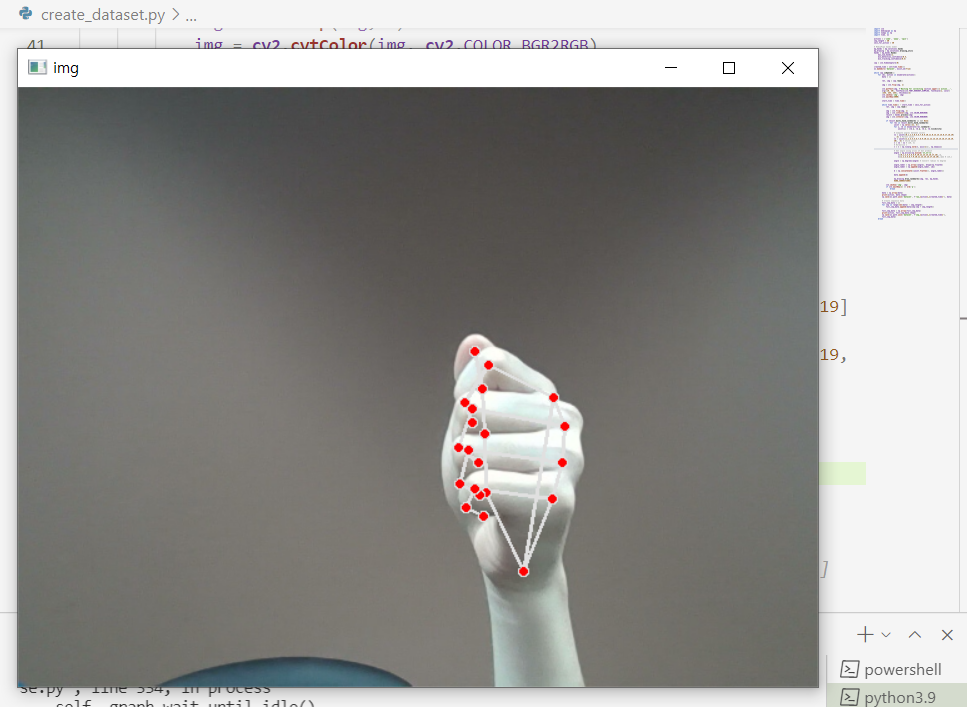
\includegraphics[width=0.8\columnwidth]{aa.png}
    \end{figure}
\end{frame}




\begin{frame}{실제학습}
    \begin{itemize}
        \item keras로 model을 학습
    \end{itemize}
    \begin{figure}
        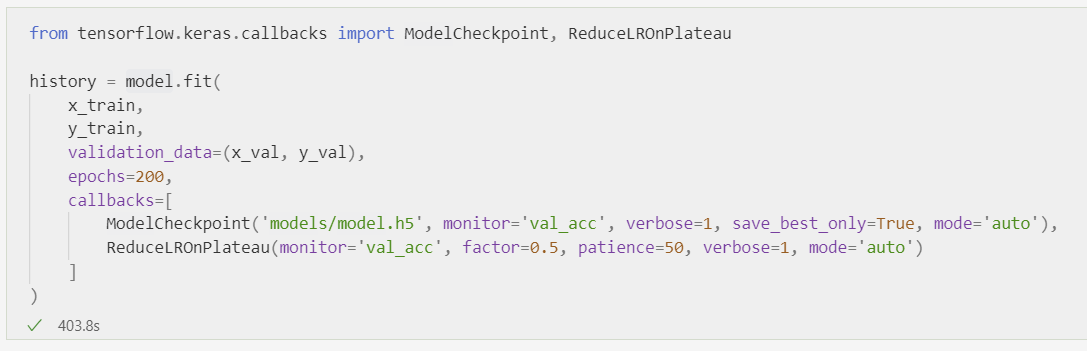
\includegraphics[width=0.8\columnwidth]{train1.png}
    \end{figure}
\end{frame}


\begin{frame}{학습 결과}
    \begin{figure}
        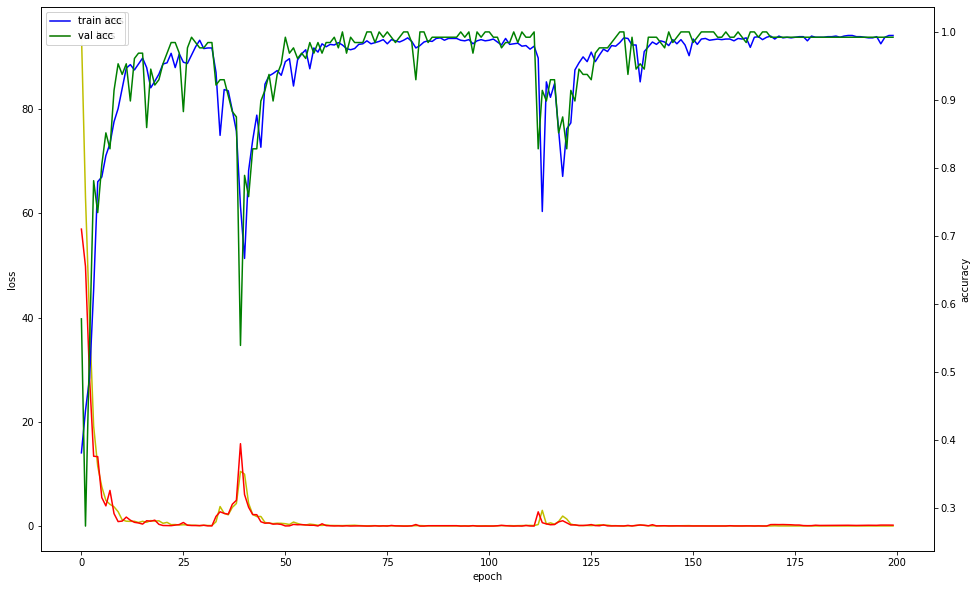
\includegraphics[width=0.9\columnwidth]{output.png}
    \end{figure}
\end{frame}


\begin{frame}{결과}
    \begin{figure}
        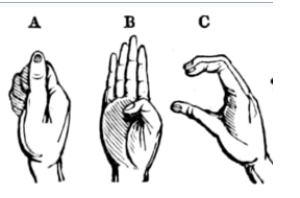
\includegraphics[width=0.8\columnwidth]{sign.png}
    \end{figure}
\end{frame}


\begin{frame}{A}
    \begin{figure}
        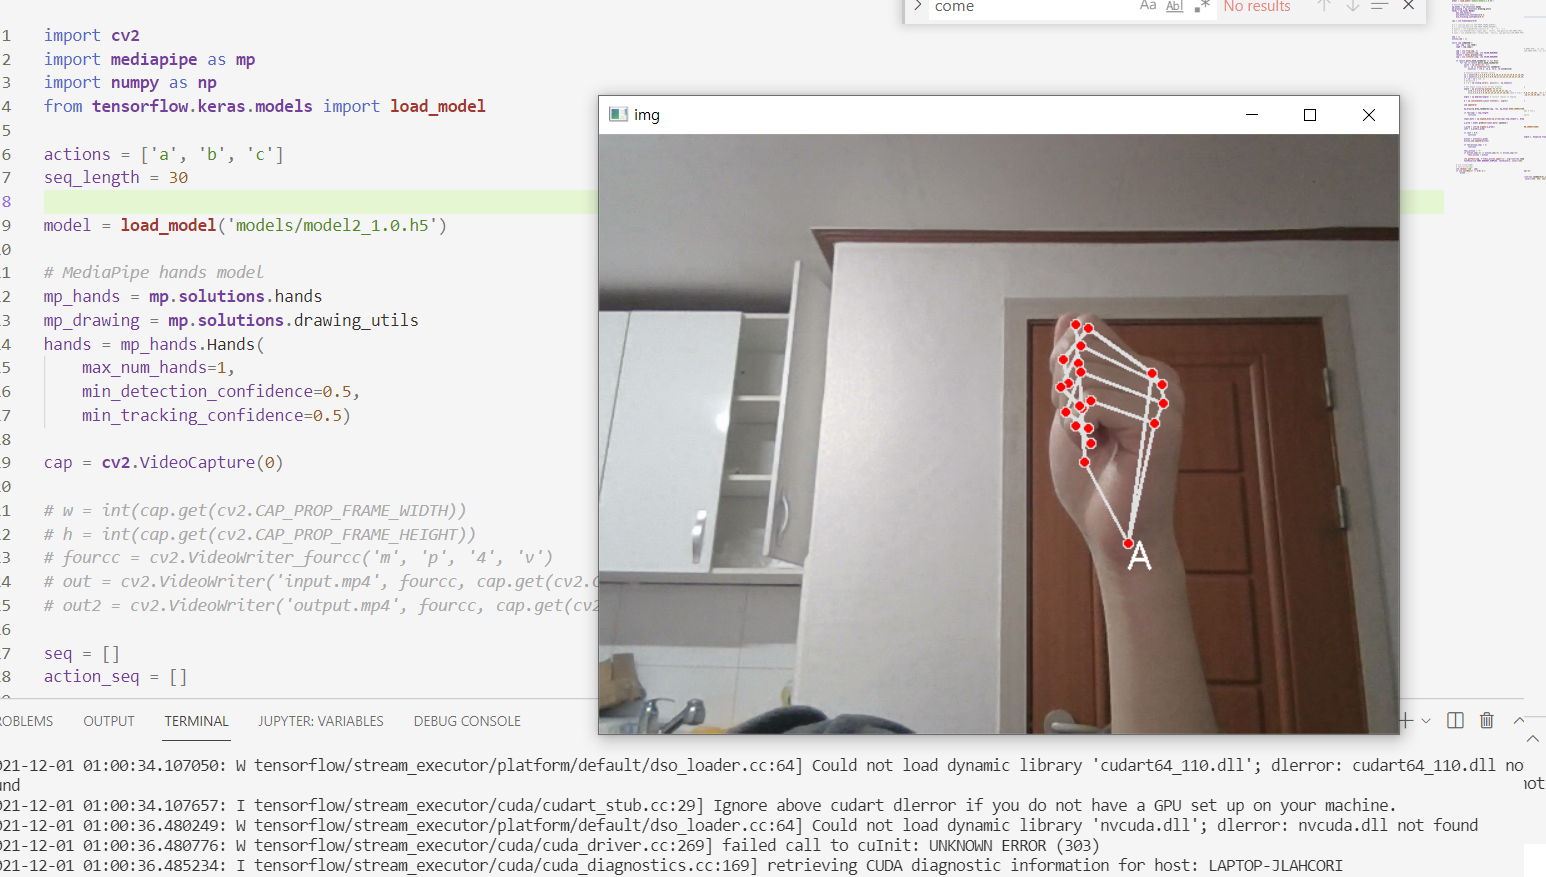
\includegraphics[width=0.8\columnwidth]{A.png}
    \end{figure}
\end{frame}

\begin{frame}{B}
    \begin{figure}
        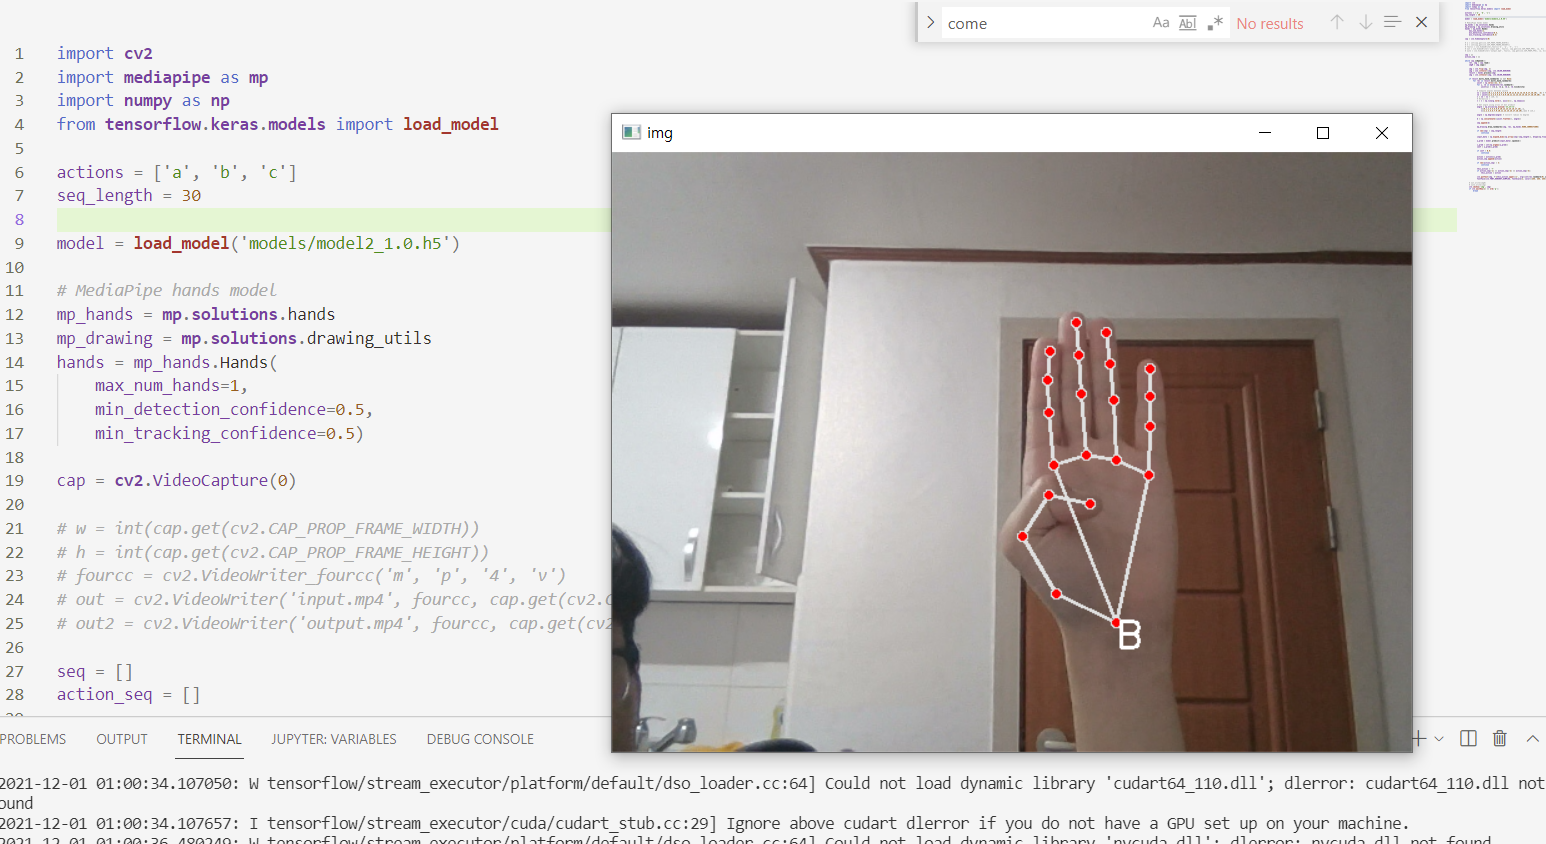
\includegraphics[width=0.8\columnwidth]{B.png}
    \end{figure}
\end{frame}

\begin{frame}{C}
    \begin{figure}
        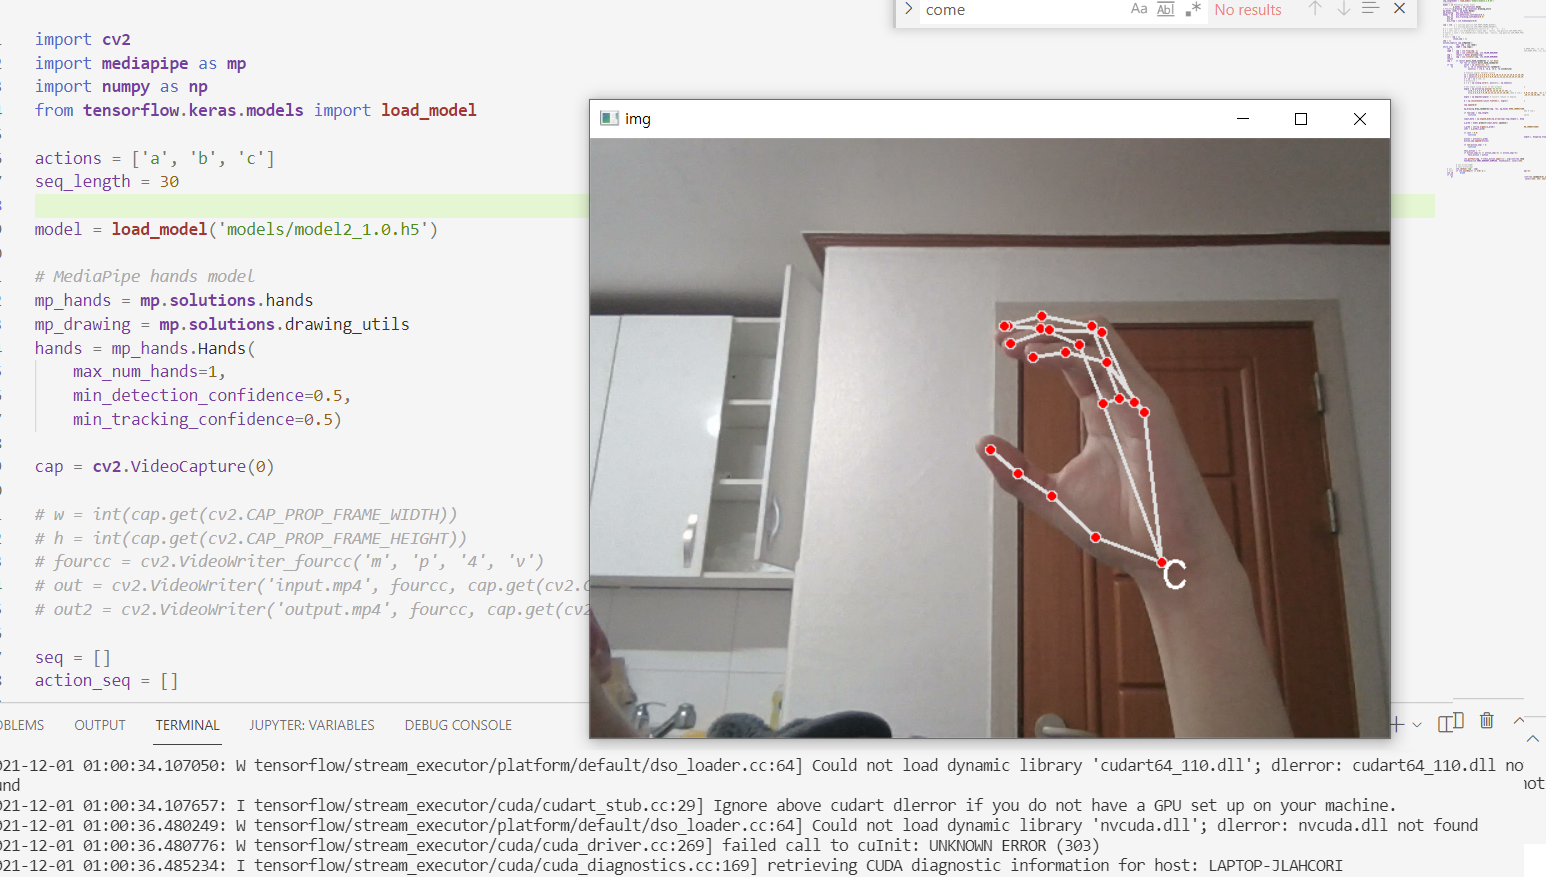
\includegraphics[width=0.8\columnwidth]{C.png}
    \end{figure}
\end{frame}



\begin{frame}{문제점}
    \begin{itemize}
        \item A,B의 인식률은 괜찮지만 C의 인식률이 별로 좋지못함.
    \end{itemize}
\end{frame}




\begin{frame}{간트차트}
    \begin{figure}
        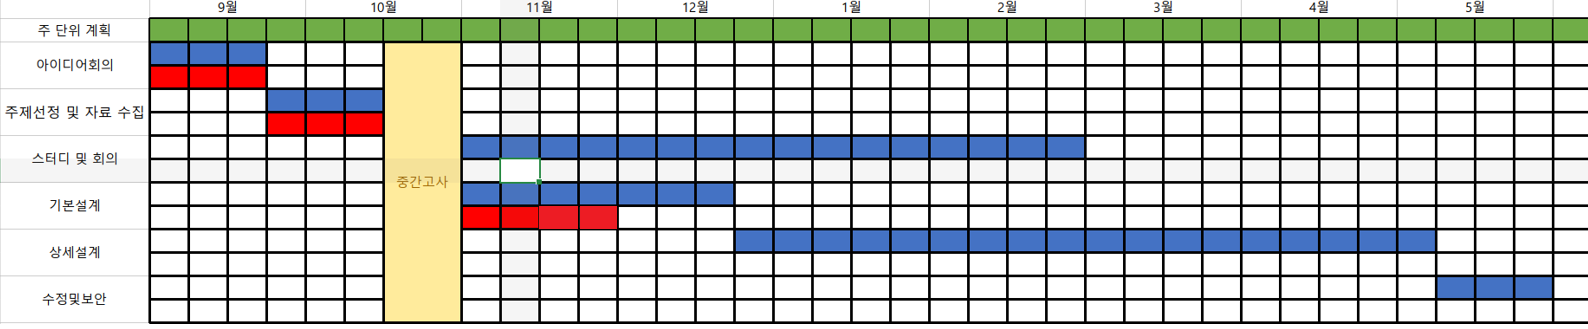
\includegraphics[width=1\columnwidth]{gant.png}
    \end{figure}
\end{frame}

\begin{frame}{앞으로 할것}
    \begin{itemize}
        \item 학습 결과 인식률이 좋지않은것을 어떻게 해야할지가 고민.
        \item 또한 머신러닝 학습 코드들을 제대로 이해하고 테스트 한것이 아니라 코드를 고치기 위해서라도 정확한 이해가 필요함
        \item 이 코드들은 앞 발표에서 사용한 가위바위보 레포와의 연관성을 찾아 둘다 활용할 수 있는 방안을 찾아봐야함.
        \item 실제 캡스톤 구현을 한다면 속도를 위해서 c++로 재작성을 해보는것도 염두.
    \end{itemize}
\end{frame}

\end{document}